\documentclass[12pt, a4paper, oneside]{ctexart}
\usepackage{amsmath, amsthm, amssymb, bm, color, graphicx, geometry, mathrsfs,extarrows, braket, booktabs, array, xcolor, fontspec, appendix, float, subfigure, wrapfig, enumitem, titlesec}
\usepackage[colorlinks,linkcolor=red,anchorcolor=blue,citecolor=blue,urlcolor=blue,menucolor=black]{hyperref}

%%%% 设置中文字体 %%%%
% fc-list -f "%{family}\n" :lang=zh >d:zhfont.txt 命令查看已有字体
\setCJKmainfont[
    BoldFont=方正黑体_GBK,  % 黑体
    ItalicFont=方正楷体_GBK,  % 楷体
    BoldItalicFont=方正粗楷简体,  % 粗楷体
    Mapping = fullwidth-stop  % 将中文句号“.”全部转化为英文句号“.”,
]{方正书宋简体}  % !!! 注意在Windows中运行请改为“方正书宋简体.ttf” !!!
%%%% 设置英文字体 %%%%
\setmainfont{Minion Pro}
\setsansfont{Calibri}
\setmonofont{Consolas}

%%%% 设置代码块 %%%%
% 在vscode中使用minted需要先配置python解释器, Ctrl+Shift+P, 输入Python: Select Interpreter选择安装了Pygments的Python版本. 再在setting.json中xelatex和pdflatex的参数中加入 "--shell-escape", 即可
% TeXworks中配置方法参考: https://blog.csdn.net/RobertChenGuangzhi/article/details/108140093
\usepackage{minted}
\renewcommand{\theFancyVerbLine}{
    \sffamily\textcolor[rgb]{0.5,0.5,0.5}{\scriptsize\arabic{FancyVerbLine}}} % 修改代码前序号大小
% 加入不同语言的代码块
\newmintinline{cpp}{fontsize=\small, linenos, breaklines, frame=lines}
\newminted{cpp}{fontsize=\small, baselinestretch=1, linenos, breaklines, frame=lines}
\newmintedfile{cpp}{fontsize=\small, baselinestretch=1, linenos, breaklines, frame=lines}
\newmintinline{matlab}{fontsize=\small, linenos, breaklines, frame=lines}
\newminted{matlab}{fontsize=\small, baselinestretch=1, mathescape, linenos, breaklines, frame=lines}
\newmintedfile{matlab}{fontsize=\small, baselinestretch=1, linenos, breaklines, frame=lines}
\newmintinline{python}{fontsize=\small, linenos, breaklines, frame=lines, python3}  % 使用\pythoninline{代码}
\newminted{python}{fontsize=\small, baselinestretch=1, linenos, breaklines, frame=lines, python3}  % 使用\begin{pythoncode}代码\end{pythoncode}
\newmintedfile{python}{fontsize=\small, baselinestretch=1, linenos, breaklines, frame=lines, python3}  % 使用\pythonfile{代码地址}

%%%% 设置行间距与页边距 %%%%
\linespread{1.2}
\geometry{left=2.5cm, right=2.5cm, top=2.5cm, bottom=2.5cm}
% \geometry{left=1.84cm,right=1.84cm,top=2.18cm,bottom=2.18cm}  % 更小的页边距

%%%% 定理类环境的定义 %%%%
\newtheorem{example}{例}            % 整体编号
\newtheorem{theorem}{定理}[section] % 定理按section编号
\newtheorem{definition}{定义}
\newtheorem{axiom}{公理}
\newtheorem{property}{性质}
\newtheorem{proposition}{命题}
\newtheorem{lemma}{引理}
\newtheorem{corollary}{推论}
\newtheorem{condition}{条件}
\newtheorem{conclusion}{结论}
\newtheorem{assumption}{假设}
\numberwithin{equation}{section}  % 公式按section编号 (公式右端的小括号)
\newtheorem{algorithm}{算法}

%%%% 自定义环境 %%%%
\newsavebox{\nameinfo}
\newenvironment{myTitle}[1]{
    \begin{center}
    {\zihao{-2}\bf #1\\}
    \zihao{-4}\it
}{\end{center}}  % \begin{myTitle}{标题内容}作者信息\end{myTitle}
\newcounter{problem}  % 问题序号计数器
\newenvironment{problem}[1][]{\stepcounter{problem}\par\noindent\textbf{题目\arabic{problem}. #1}}{\smallskip\par}
\newenvironment{solution}[1][]{\par\noindent\textbf{#1解答. }}{\smallskip\par}  % 可带一个参数表示题号\begin{solution}{题号}
\newenvironment{note}{\par\noindent\textbf{注记. }}{\smallskip\par}
\newenvironment{remark}{\begin{enumerate}[label=\textbf{注\arabic*.}]}{\end{enumerate}}
\BeforeBeginEnvironment{minted}{\vspace{-0.5cm}}  % 缩小minted环境距上文间距
\AfterEndEnvironment{minted}{\vspace{-0.2cm}}  % 缩小minted环境距下文间距

%%%% 自定义段落开头序号,间距 (titlesec) %%%%
% 中文序号:\zhnum{section}, 阿拉伯序号:\arabic
\titleformat{\section}{\Large\bfseries}{\arabic{section}}{1em}{}[]
\titlespacing{\section}{0pt}{1.2ex plus .0ex minus .0ex}{.6ex plus .0ex}
\titlespacing{\subsection}{0pt}{1.2ex plus .0ex minus .0ex}{.6ex plus .0ex}
\titlespacing{\subsubsection}{0pt}{1.2ex plus .0ex minus .0ex}{.6ex plus .0ex}

%%%% 图片相对路径 %%%%
\graphicspath{{figures/}} % 当前目录下的figures文件夹, {../figures/}则是父目录的figures文件夹
\setlength{\abovecaptionskip}{-0.2cm}  % 缩紧图片标题与图片之间的距离
\setlength{\belowcaptionskip}{0pt} 

%%%% 缩小item,enumerate,description两行间间距 %%%%
\setenumerate[1]{itemsep=0pt,partopsep=0pt,parsep=\parskip,topsep=5pt}
\setitemize[1]{itemsep=0pt,partopsep=0pt,parsep=\parskip,topsep=5pt}
\setdescription{itemsep=0pt,partopsep=0pt,parsep=\parskip,topsep=5pt}

%%%% 自定义公式 %%%%
\everymath{\displaystyle} % 默认全部行间公式, 想要变回行内公式使用\textstyle
\DeclareMathOperator*\uplim{\overline{lim}}     % 定义上极限 \uplim_{}
\DeclareMathOperator*\lowlim{\underline{lim}}   % 定义下极限 \lowlim_{}
\DeclareMathOperator*{\argmax}{arg\,max}  % 定义取最大值的参数 \argmax_{}
\DeclareMathOperator*{\argmin}{arg\,min}  % 定义取最小值的参数 \argmin_{}
\let\leq=\leqslant % 简写小于等于\leq (将全部leq变为leqslant)
\let\geq=\geqslant % 简写大于等于\geq (将全部geq变为geqslant)
\DeclareRobustCommand{\rchi}{{\mathpalette\irchi\relax}}
\newcommand{\irchi}[2]{\raisebox{\depth}{$#1\chi$}} % 使用\rchi将\chi居中

%%%% 一些宏定义 %%%%
\def\bd{\boldsymbol}        % 加粗(向量) boldsymbol
\def\disp{\displaystyle}    % 使用行间公式 displaystyle(默认)
\def\tsty{\textstyle}       % 使用行内公式 textstyle
\def\sign{\text{sign}}      % sign function
\def\wtd{\widetilde}        % 宽波浪线 widetilde
\def\R{\mathbb{R}}          % Real number
\def\N{\mathbb{N}}          % Natural number
\def\Z{\mathbb{Z}}          % Integer number
\def\Q{\mathbb{Q}}          % Rational number
\def\C{\mathbb{C}}          % Complex number
\def\K{\mathbb{K}}          % Number Field
\def\P{\mathbb{P}}          % Polynomial
\def\E{\mathbb{E}}          % Exception
\def\d{\mathrm{d}}          % differential operator
\def\e{\mathrm{e}}          % Euler's number
\def\i{\mathrm{i}}          % imaginary number
\def\re{\mathrm{Re}}        % Real part
\def\im{\mathrm{Im}}        % Imaginary part
\def\res{\mathrm{Res}}      % Residue
\def\ker{\mathrm{Ker}}      % Kernel
\def\vspan{\mathrm{vspan}}  % Span  \span与latex内核代码冲突改为\vspan
\def\L{\mathcal{L}}         % Loss function
\def\O{\mathcal{O}}         % big O notation
\def\wdh{\widehat}          % 宽帽子 widehat
\def\ol{\overline}          % 上横线 overline
\def\ul{\underline}         % 下横线 underline
\def\add{\vspace{1ex}}      % 增加行间距
\def\del{\vspace{-1.5ex}}   % 减少行间距

%%%% 正文开始 %%%%
\begin{document}

%%%% 以下部分是正文 %%%%  
\begin{myTitle}{第一次作业\quad 测试VAE拓展模型生成效果}
    生成式人工智能\\ 吴天阳\ 4124136039\ 人工智能B2480
\end{myTitle}
\section{应用实践}
使用CVAE模型在FashionMNIST数据集上进行训练,以下是各模块代码

\subsection{模型定义}

本实验使用MLP与卷积分别搭建两个模型。MLP模型以展平后的784维MNIST图像向量与10维one-hot标签向量直接拼接作为输入,
编码器通过512维隐层进行特征融合后,并行输出潜在空间的均值与对数方差参数。解码阶段将64维潜在向量与条件标签拼接,经相同维度的全连接层映射后,
通过Sigmoid激活重构$28\times 28$像素图像。该架构通过向量级拼接实现条件信息的显式融合,编码阶段采用单隐层结构简化特征提取流程,解码过程通过全连接网络的全局感知特性实现图像整体结构的生成。

卷积架构CVAE模型输入为$28\times 28$灰度图像与10维one-hot标签的融合信息:编码阶段将标签张量沿空间维度扩展至与图像同尺寸后拼接于通道维度,
形成11通道的复合输入,经过两次步长为2的卷积下采样($32\to 64$通道)获得$7\times 7$特征图,最终通过全连接层输出潜在空间的均值与对数方差。
解码阶段将潜在向量与条件标签拼接后,经全连接层恢复至$64\times 7\times 7$特征维度,通过两层转置卷积完成上采样重构,输出层采用Sigmoid激活确保像素值在$[0,1]$区间。
\pythonfile{CVAE.py}
\subsection{训练结果}
分别训练两个模型各50个epochs,进行模型图像生成,重构,以及平滑度测试,测试结果如下
\subsubsection{MLP模型}
\begin{figure}[htbp]
    \centering
    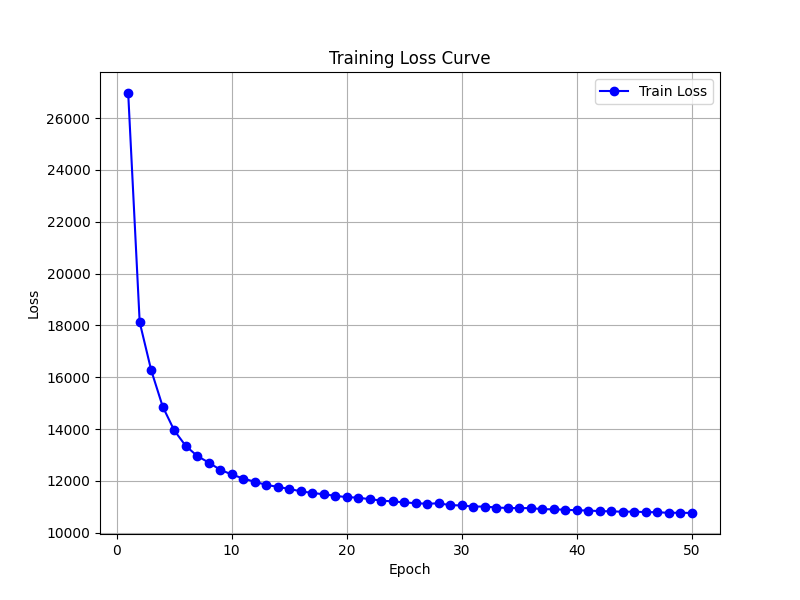
\includegraphics[width=0.8\linewidth]{hw1_mlp_loss.png}
    \caption{MLP训练损失函数曲线}
\end{figure}
\begin{figure}[htbp]
  \centering
  \subfigure[图像生成]{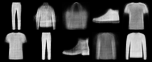
\includegraphics[width=0.49\textwidth]{hw1_mlp_generate.png}}
  \subfigure[图像重构]{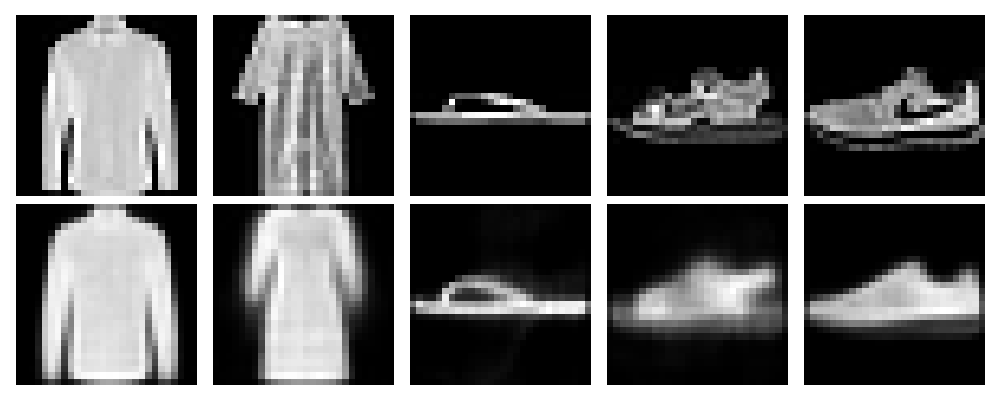
\includegraphics[width=0.49\textwidth]{hw1_mlp_reconstruct.png}}
  \setlength{\abovecaptionskip}{0ex}  % 如果使用了minted会增大图像与标题间距需要进行缩小
  \label{fig-1}
  \caption{重构图像效果}
\end{figure}
\begin{figure}[htbp]
    \centering
    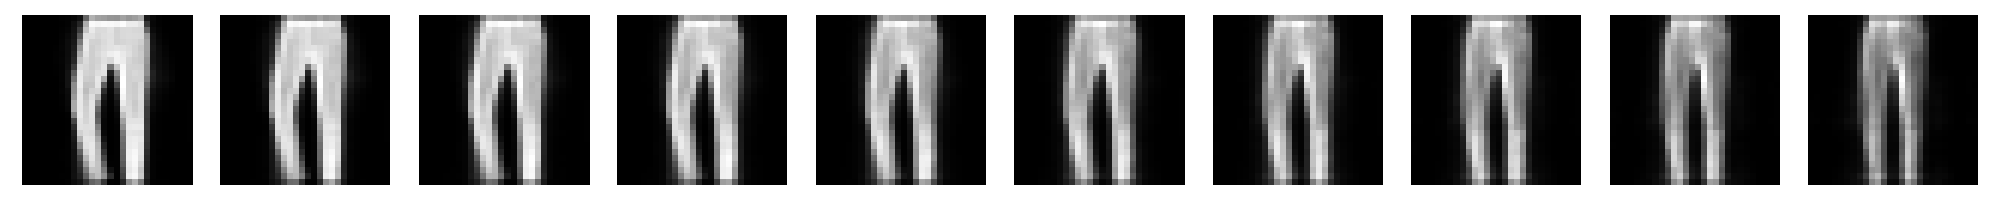
\includegraphics[width=\linewidth]{hw1_mlp_smooth_test.png}
    \caption{隐空间连续差值采样}
\end{figure}
\subsubsection{卷积模型}
\begin{figure}[htbp]
    \centering
    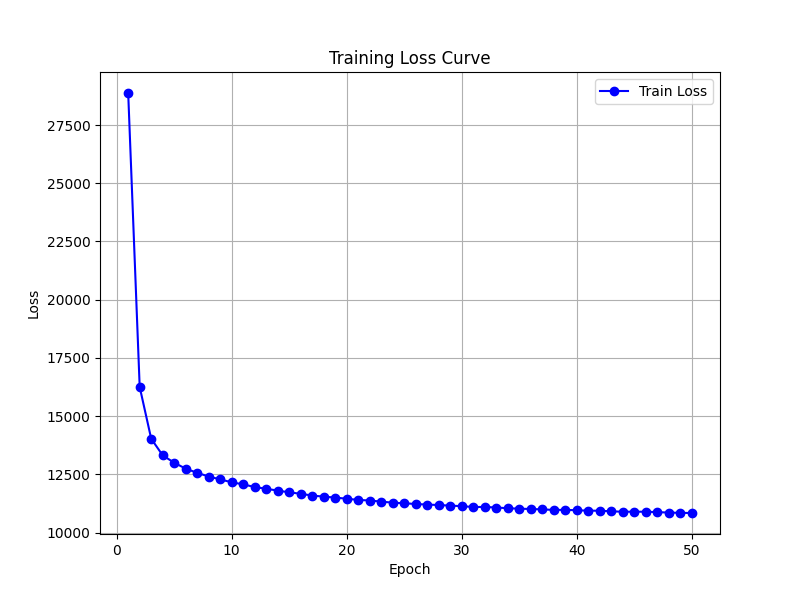
\includegraphics[width=0.8\linewidth]{hw1_cnn_loss.png}
    \caption{CNN训练损失函数曲线}
\end{figure}
\begin{figure}[htbp]
  \centering
  \subfigure[图像生成]{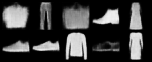
\includegraphics[width=0.49\textwidth]{hw1_cnn_generate.png}}
  \subfigure[图像重构]{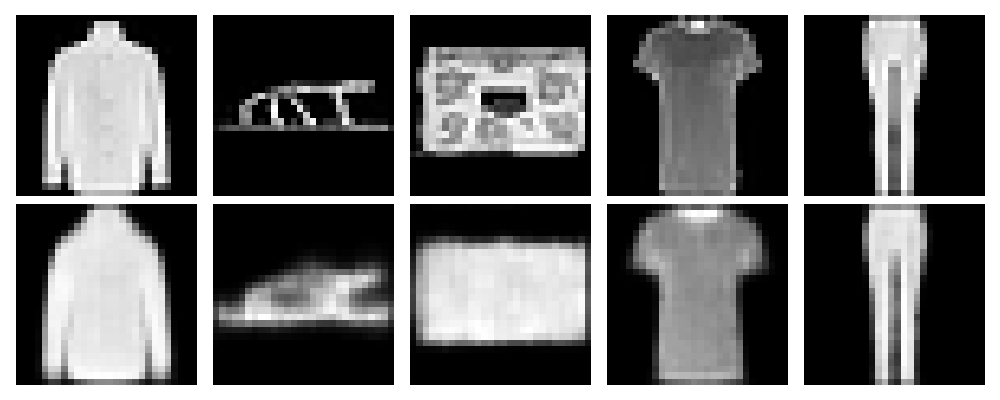
\includegraphics[width=0.49\textwidth]{hw1_cnn_reconstruct.png}}
  \setlength{\abovecaptionskip}{0ex}  % 如果使用了minted会增大图像与标题间距需要进行缩小
  \label{fig-1}
  \caption{重构图像效果}
\end{figure}
\begin{figure}[htbp]
    \centering
    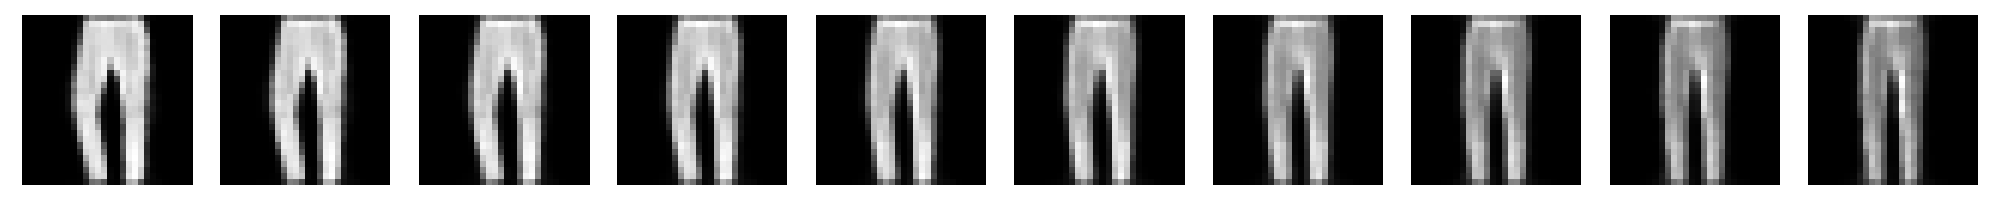
\includegraphics[width=\linewidth]{hw1_cnn_smooth_test.png}
    \caption{隐空间连续差值采样}
\end{figure}
可以发现卷积结构CVAE拥有与MLP结构相同的效果,而模型大小从MLP的3.5M下降到2.8M,更加轻量化。
\section{理论分析}
\subsection{先验分布与隐空间结构化}
VAE假设潜在变量z服从标准高斯先验,这一选择具有多重理论意义:
\begin{itemize}
    \item 几何正则性:各向同性高斯分布强制潜在空间满足局部连续性,使得解码器的微小扰动对应生成结果的平滑过渡
    \item 计算可行性:高斯分布的KL散度具有闭合解,极大简化优化过程
    \item 信息瓶颈作用:通过KL项约束隐变量携带信息量,防止模型退化为确定性自编码器
\end{itemize}
\subsection{近似后验分布与推断网络}
编码器作为高斯近似后验的参数化形式,其设计隐含以下理论权衡:
\begin{itemize}
    \item 表达能力限制:假设虽简化计算,但忽略变量间相关性,导致后验坍塌风险
    \item 变分间隙分析:真实后验与近似后验的KL散度构成ELBO目标的下界间隙,直接影响模型容量
    \item 重参数化技巧:通过实现梯度回传,本质是路径导数在连续分布场景的应用
\end{itemize}
\subsection{高斯假设的深层影响}
(1) 解码器输出建模

对于图像数据,常假设或伯努利分布。这种选择导致:
\begin{itemize}
    \item 像素独立性假设:忽略像素间空间相关性,生成图像常出现模糊现象
    \item 似然函数局限性:L2重构损失与人类感知差异的不匹配性,促使后续研究转向对抗训练(如VAE-GAN)
\end{itemize}
(2) 隐变量非线性纠缠

虽然高斯先验强制隐空间局部线性,但解码器的深度非线性变换导致:
\begin{itemize}
    \item 流形学习视角:VAE本质学习从潜空间到数据流形的可微映射,高斯先验对应流形上的均匀测度
    \item 解耦表示困境:标准高斯先验难以自然产生解耦表征,需引入解耦正则项(如β-VAE)
\end{itemize}
\end{document}
